
We show that our model produces accurate and more calibrated probabilistic forecast compared to baseline models on one synthetic and two real world trajectory prediction datasets: interacting particles, autonomous vehicle, and pedestrian movement. 
\subsection{Baselines}
%We compare our model PECCO against the following baselines:
\begin{itemize}
\itemsep0em 
   \item \texttt{LSTM-NLL} (variation of \cite{sociallstm}): An encoder-decoder LSTM model that predicts the mean and variance of a Gaussian distribution, optimizing likelihood of data. We also train a version with random rotation data augmentation \texttt{LSTM-aug}.
    \item \texttt{CtsConv} \cite{ummenhofer2019lagrangian}: Continuous convolution over point cloud data for trajectory prediction, a non-equivariant counterpart of PECCO. \texttt{CtsConv-aug} is trained with a data augmentation step where we randomly rotate the scenes. 
    %\item \texttt{ECCO} \cite{ecco}: State-of-the-art equivariant model for deterministic trajectory prediction. 
     \item \texttt{Multiple Futures Prediction (MFP)} \cite{mfp}: A encoder-decoder model for multimodal probabilistic trajectory forecasts.
     \item \texttt{Trajectron++} \cite{trajectron++}: State-of-the-art probabilistic trajectory prediction model with graph representation of agent interactions and conditional VAE architecture.
\end{itemize}
% For the deterministic models (\texttt{LSTM}, \texttt{CtsConv}), we modify them by training with Negative Log-Likelihood (NLL) and Mean Regional Score (MRS) as loss functions, the results for the deterministic baselines are in Appendix \ref{app:deterministic}.
%   \item \texttt{LSTM-NLL}: Encoder-decoder LSTM network trained optimizing mean negative log loss. Model only the agent / primary pedestrian.
%     \item \texttt{LSTM-MRS}:  Encoder-decoder LSTM network trained with mean regional score.
%     \item \texttt{LSTM-NLL-r}: Similar to LSTM-NLL, but with trajectory data rotated to face the same direction.
%     \item \texttt{LSTM-aug-r}: Similar to LSTM-MRS, but with trajectory data rotated to face the same direction.
%     \item \texttt{CtsConv-NLL}: Probabilistic continuous convolution trained with negative log-likelihood loss. It is non-equivariant counterpart of PECCO.
%     \item \texttt{CtsConv-MRS}: Probabilistic continuous convolution model trained with mean regional score loss.
%     \item \texttt{CtsConv-NLL-Aug}: Similar to CtsConv-NLL, with training data augmented by rotating the scenes by random angles.

\subsection{Evaluation Metrics.}
\begin{itemize}%[noitemsep, leftmargin=*]
\itemsep0em 
\item \textit{Minimum Average/Final Displacement Error} (minADE$_6$, minFDE$_6$):  average $l_2$ displacement error over $k$ steps, or average displacement of the final step, between predicted and ground truth trajectories. We report the minimum over 6 samples for probabilistic models. 
\item \textit{Negative Log Likelihood} (NLL): NLL of ground truth trajectories under predicted distributions.
%\item \textit{Mean Regional Score} (MRS): Score function for confidence region prediction introduced in \autoref{eq:mrs}. We report MRS for $\alpha=0.1$, the 90\% cofidence region. 
\item \textit{Energy Score} (ES) \cite{properscoring}: a proper scoring rule to measure calibration and sharpness of the predicted distribution $P$. The energy score for a distribution $P$ and the ground truth data $x$ is defined as: $\text{ES}(P, x) = E_{X \sim P} \| X - x \| - \frac{1}{2} E_{ X, X' \sim P} \| X - X' \| $. Here $X$ and $X'$ are independent samples from $P$. 
\item \textit{Coverage}: The empirical estimate of probability of the true value lying in the predicted interval, defined in  \eqref{eq:coverage}. We report the coverage of 90\% quantile of the predicted Gaussian. The  prediction is more \textit{calibrated} if the coverage is closer to 90\%.
\end{itemize}

% \subsection{Argoverse Motion Forecasting Dataset}
\subsection{Datasets.}
The particle dataset is a synthetic dataset of 5 particles interacting in spring dynamics \cite{nri} with dynamics noise. The models predict 20 time steps given 30 steps as input.
The Argoverse autonomous vehicle motion forecasting \cite{argoverse} is a widely used vehicle trajectory prediction benchmark. The task is to predict 3 second trajectories based on all vehicle history in the past 2 seconds recorded at 10Hz. 
%
TrajNet++ \cite{pedestriandata} is a popular pedestrian trajectory benchmark with a focus on agent-agent interaction scenarios. The task is to predict 12 time steps for agents given 9. We refer the reader to Appendix \ref{app:exp} for data and training details. 

%PECCO predicts all agents' trajectories jointly. The metrics for particle dataset is averaged over 5 particles. Following literature, we report on metrics for the agent vehicle (Argoverse) and primary pedestrian (TrajNet++). 
\subsection{Experimental Results}

\begin{table}
\centering
    \begin{tabular}{c|c c c}
     \toprule
  \textbf{Model} & MSE $\downarrow$ & NLL$\downarrow$  & ES  $\downarrow$\\ 
  \midrule
  LSTM & .016 &  -1.61 & 1.041 \\
  %Conditional Flow & .288 &  -0.42 & 0.928 \\
  CtsConv & .010 &  -0.81  & 0.667 \\
  PECCO & \textbf{.004} & \textbf{-0.83} & \textbf{0.467} \\
    \bottomrule
    \end{tabular}
\caption{PECCO outperforms baseline models in all metrics on the synthetic particles dataset. }
\label{tab:particles}
\end{table}

\begin{table}[t!]
\centering   \resizebox{\textwidth}{!}{
\begin{tabular}{ c|c c c c | ccc } 
 \toprule
  \textbf{Model} & minADE${}_6 \downarrow$ & minFDE${}_6 \downarrow$ & NLL$\downarrow$ & ES $\downarrow$& Cov@1s(\%) & Cov@2s & Cov@3s\\ 
\midrule
 \multicolumn{8}{c}{Argoverse}\\
 \midrule
LSTM-NLL   & 1.64 \plusminus{.05} & 4.17 \plusminus{.10} & 3.07 \plusminus{.08} & 2.31 \plusminus{.54} & 8.8 \plusminus{0.7} & 8.5 \plusminus{0.7} & 7.0 \plusminus{0.8} \\
LSTM-NLL-aug    & 1.61 \plusminus{.02} & 4.15 \plusminus{.08} & 2.78 \plusminus{.03} & 1.99 \plusminus{.46} & 10.1 \plusminus{1.5} & 10.5 \plusminus{1.0} & 9.8 \plusminus{1.9} \\
CtsConv-NLL  & 1.74 \plusminus{.03} & 4.43 \plusminus{.06} & 29.1 \plusminus{2.2} & 6.71 \plusminus{.70} & 6.3 \plusminus{2.2} & 0.02 \plusminus{.01} & 0.01 \plusminus{.01}\\
CtsConv-NLL-aug  & 1.66 \plusminus{.02} & 4.23 \plusminus{.06} & 11.81 \plusminus{.01} & 5.10 \plusminus{.35} & 11.9 \plusminus{2.1} & 1.7 \plusminus{0.5} & 0.02 \plusminus{.01} \\
Trajectron++   & 1.83 \plusminus{.02} & 3.85 \plusminus{.07} & \textbf{2.48} \plusminus{.27} & 3.92  \plusminus{.61} & 45.5 \plusminus{5.3} & 37.6 \plusminus{3.2}  & 34.9 \plusminus{2.5} \\
MFP  & 1.53 \plusminus{.04} & 3.77 \plusminus{.06} & 3.56 \plusminus{.02} & 2.33 \plusminus{.21} & 51.3 \plusminus{5.1} & 33.0 \plusminus{4.9} & 8.3 \plusminus{4.8} \\
\midrule
PECCO   & \textbf{1.39} \plusminus{.02}  & \textbf{3.41} \plusminus{.03} & 4.26 \plusminus{0.1} & \textbf{1.54} \plusminus{.16} & \textbf{74.9} \plusminus{0.6} & \textbf{78.6} \plusminus{2.8} & \textbf{84.5} \plusminus{2.9}\\
% \bottomrule
% \end{tabular}
% \caption{Performance comparison on the Argoverse dataset}
% \label{tab:arg-baseline}
% \end{table*}
% \begin{table*}[h]
% \centering
% \begin{tabular}{ c|c c c c|c c c } 
\toprule
 \multicolumn{8}{c}{TrajNet++}\\
%   \textbf{Model} & minADE${}_6 \downarrow$ & minFDE${}_6 \downarrow$ & NLL$\downarrow$ & MRS  $\downarrow$& Cov@4(\%) & Cov@8 & Cov@12\\ 
  \midrule
LSTM-NLL-aug & 0.85 \plusminus{.02} & 1.64 \plusminus{.03} & 2.78 \plusminus{.02} & -0.28 \plusminus{.09}  & 29.0 \plusminus{4.3} & 23.2 \plusminus{4.2} & 23.7\plusminus{3.9} \\
% LSTM-MRS-r  & 0.94 \plusminus{.01} & 1.84 \plusminus{.02} & 123.7 \plusminus{5.0} & \textbf{3.3} \plusminus{0.1} & 95.7 \plusminus{5.2} & \textbf{94.3} \plusminus{5.6} & 96.5 \plusminus{3.4} \\
CtsCov-NLL & 1.08 \plusminus{.02} & 2.36 \plusminus{.09} & 5.33 \plusminus{.08} & 1.67 \plusminus{.13}  & 43.8 \plusminus{10.6}  & 20.7 \plusminus{5.2} & 12.2 \plusminus{6.7} \\
% CtsConv-MRS & 0.96 \plusminus{.02} & 2.28 \plusminus{.07} & 5.97 \plusminus{.20} & 8.2 \plusminus{0.9} & \textbf{93.4} \plusminus{5.2} & 64.5 \plusminus{5.2} & 46.1 \plusminus{4.8} \\
CtsCov-NLL-aug &  0.92 \plusminus{.01 } & 1.76 \plusminus{.03} & 6.74 \plusminus{.21} & 1.42 \plusminus{.11}  & 62.1 \plusminus{3.3}  & 36.3 \plusminus{4.9} & 34.1 \plusminus{5.8} \\
Trajectron++  & 1.14 \plusminus{.03} & 2.31 \plusminus{.05} & 2.83 \plusminus{.12} & 0.98 \plusminus{.17} & 50.2 \plusminus{2.2} & 45.8 \plusminus{3.5} & 32.9 \plusminus{3.5}\\
MFP & 0.85 \plusminus{.02}  & 1.70 \plusminus{.04}  & \textbf{2.20} \plusminus{.04}  & 0.67 \plusminus{.08} & 79.1 \plusminus{4.3}  & 32.5 \plusminus{3.1}  & 22.8 \plusminus{3.2} \\
\midrule
PECCO & \textbf{0.59} \plusminus{.12}  & \textbf{1.06} \plusminus{.17} & 2.37 \plusminus{.04} & \textbf{-0.73} \plusminus{.10} &  \textbf{80.8} \plusminus{4.5} &  \textbf{85.9} \plusminus{2.3} &  \textbf{94.5} \plusminus{3.0} \\
\bottomrule
\end{tabular}
}
\caption{Performance comparison on benchmark datasets Argoverse and TrajNet++. Cov@$k$s(\%) refers to coverage at the $k$ second mark; prediction is more \textit{calibrated} if closer to 90\%. PECCO is more accurate and calibrated compared to non-equivariant baseline models.} 
\label{tab:big-table}
\end{table}


\textbf{Particles dataset.} We present experimental result for the synthetic particle dataset in Table 1. We visualize a test sample in \autoref{fig:particle} to qualitatively illustrate PECCO's improved accuracy and calibration. 

\noindent \textbf{Argoverse and TrajNet++.}
\autoref{tab:big-table} presents experimental results on two benchmark datasets. PECCO achieves better regression accuracy compared to non-equivariant baseline in terms of minADE and minFDE, with a notable 9\% improvement in minADE over the the best performing baseline, MFP. PECCO's improved probability coverage allows for more diverse sampling and hence can produce trajectories closer to ground truth. 

PECCO's probabilistic predictions are able to achieve consistently better coverage compared to other methods whose coverage deteriorates over time. Comparing LSTM-NLL and CtsConv-NLL with their augmented counterparts, LSTM-NLL-aug and CtsConv-NLL-aug, we can see that data augmentation through rotation improves both accuracy and calibration. PECCO leverages this symmetry to improve accuracy, maintain good calibration, and converge faster (\autoref{fig:dataeff}).

Figure \ref{fig:arg_experiment} visualizes a typical situation to illustrate this difference. We plot the predicted distribution at 10, 20, and 30 time steps of prediction (1 time step is 0.1 seconds). We can see the probable region predicted by LSTM-NLL explodes at timesteps 20 and 30, whereas CtsConv-NLL and MFP tend to be overconfident in their predictions. PECCO is able to predict a Gaussian that covers both cases of staying in the lane and changing to the right lane. 

\begin{figure}[t]
    \centering
    \begin{subfigure}[b]{0.32\textwidth}
        \centering
        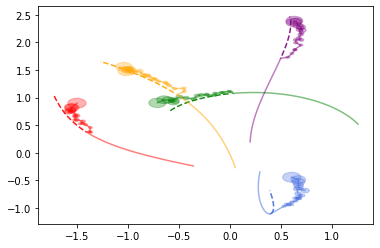
\includegraphics[width=\textwidth]{equivariance/figs/particle/lstm.png}
        \caption{LSTM}
        \label{fig:lstm}
    \end{subfigure}
    \hfill
    \begin{subfigure}[b]{0.32\textwidth}
        \centering
        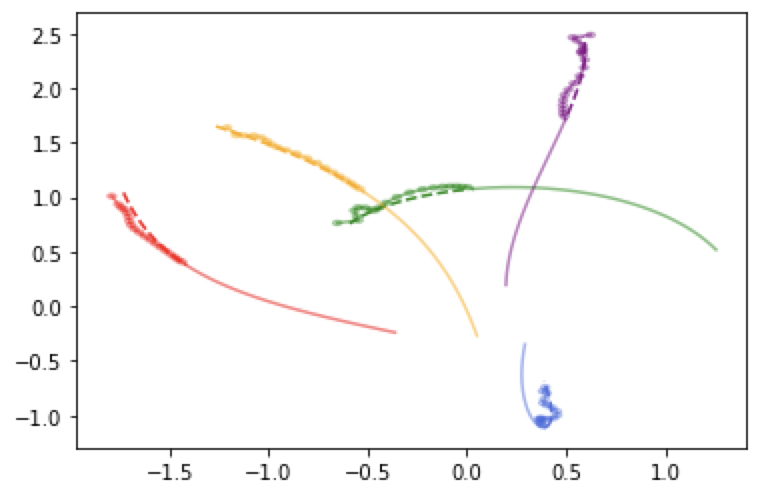
\includegraphics[width=\textwidth]{equivariance/figs/particle/ctsconv.jpg}
        \caption{CstConv}
        \label{fig:ctsconv}
    \end{subfigure}
    \hfill
    \begin{subfigure}[b]{0.32\textwidth}
        \centering
        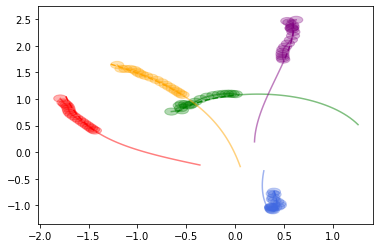
\includegraphics[width=\textwidth]{equivariance/figs/particle/pecco.png}
        \caption{PECCO}
        \label{fig:pecco}
    \end{subfigure}
    \caption{Comparison of prediction results between baselines. The solid lines are input timesteps to the models, the dotted lines ground truth, and the circles the 90\% confidence regions. We can see that PECCO achieves accurate results while maintaining good coverage.}
    \label{fig:particle}
\end{figure}


\begin{figure}[t]
\centering
\begin{subfigure}[t]{0.23\textwidth}
\centering
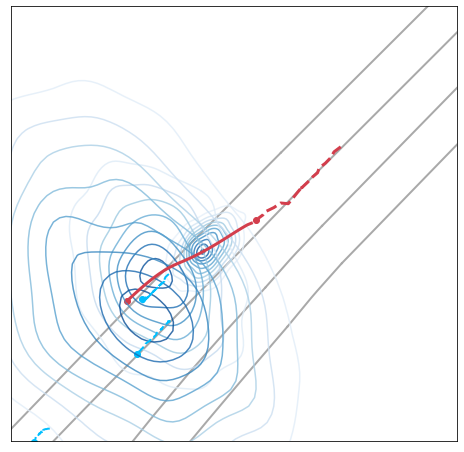
\includegraphics[width=\linewidth]{equivariance/figs/10049lstm.png}
\subcaption{LSTM-NLL}
\label{fig:sub1}
\end{subfigure}
% \begin{subfigure}[t]{0.23\textwidth}
%   \centering
%   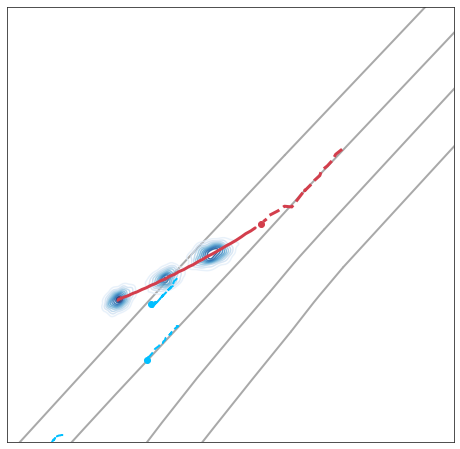
\includegraphics[width=\linewidth]{figs/10049nll.png}
%   \subcaption{CtsConv-NLL}
%   \label{fig:sub2}
% \end{subfigure}
\begin{subfigure}[t]{0.23\textwidth}
\centering
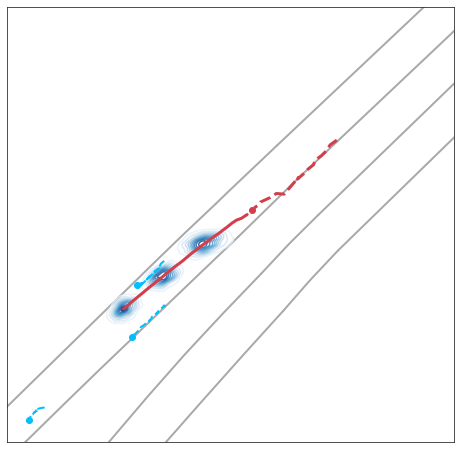
\includegraphics[width=\linewidth]{equivariance/figs/10049mis.png}
\subcaption{CtsConv-NLL}
\label{fig:sub3}
\end{subfigure}
\begin{subfigure}[t]{0.23\textwidth}
\centering
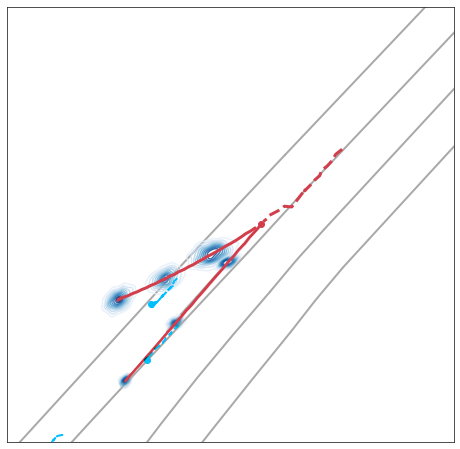
\includegraphics[width=\linewidth]{equivariance/figs/mfp.png}
\subcaption{MFP}
\label{fig:sub3a}
\end{subfigure}
\begin{subfigure}[t]{0.23\textwidth}
\centering
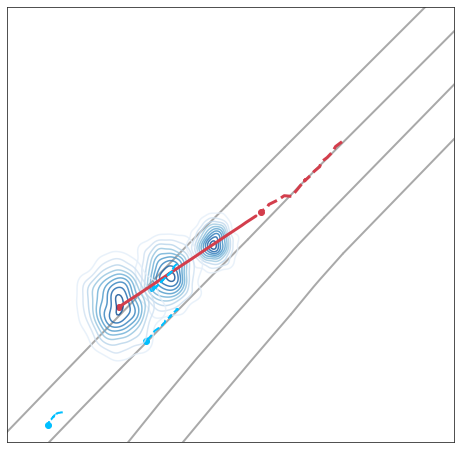
\includegraphics[width=\linewidth]{equivariance/figs/10049dyna.png}
\subcaption{PECCO}
\label{fig:sub4}
\end{subfigure}
\caption{Comparison of uncertainty predicted at a lane change. Red trajectories are the agent of interest in the same scenario. Note how the LSTM predicted uncertainty explodes after a few time steps, while CtsConv and MFP has overconfident distributions. PECCO is able to model possibility of both staying and lane change.}
\label{fig:arg-experiment}
\end{figure}

\begin{figure}
    \centering
      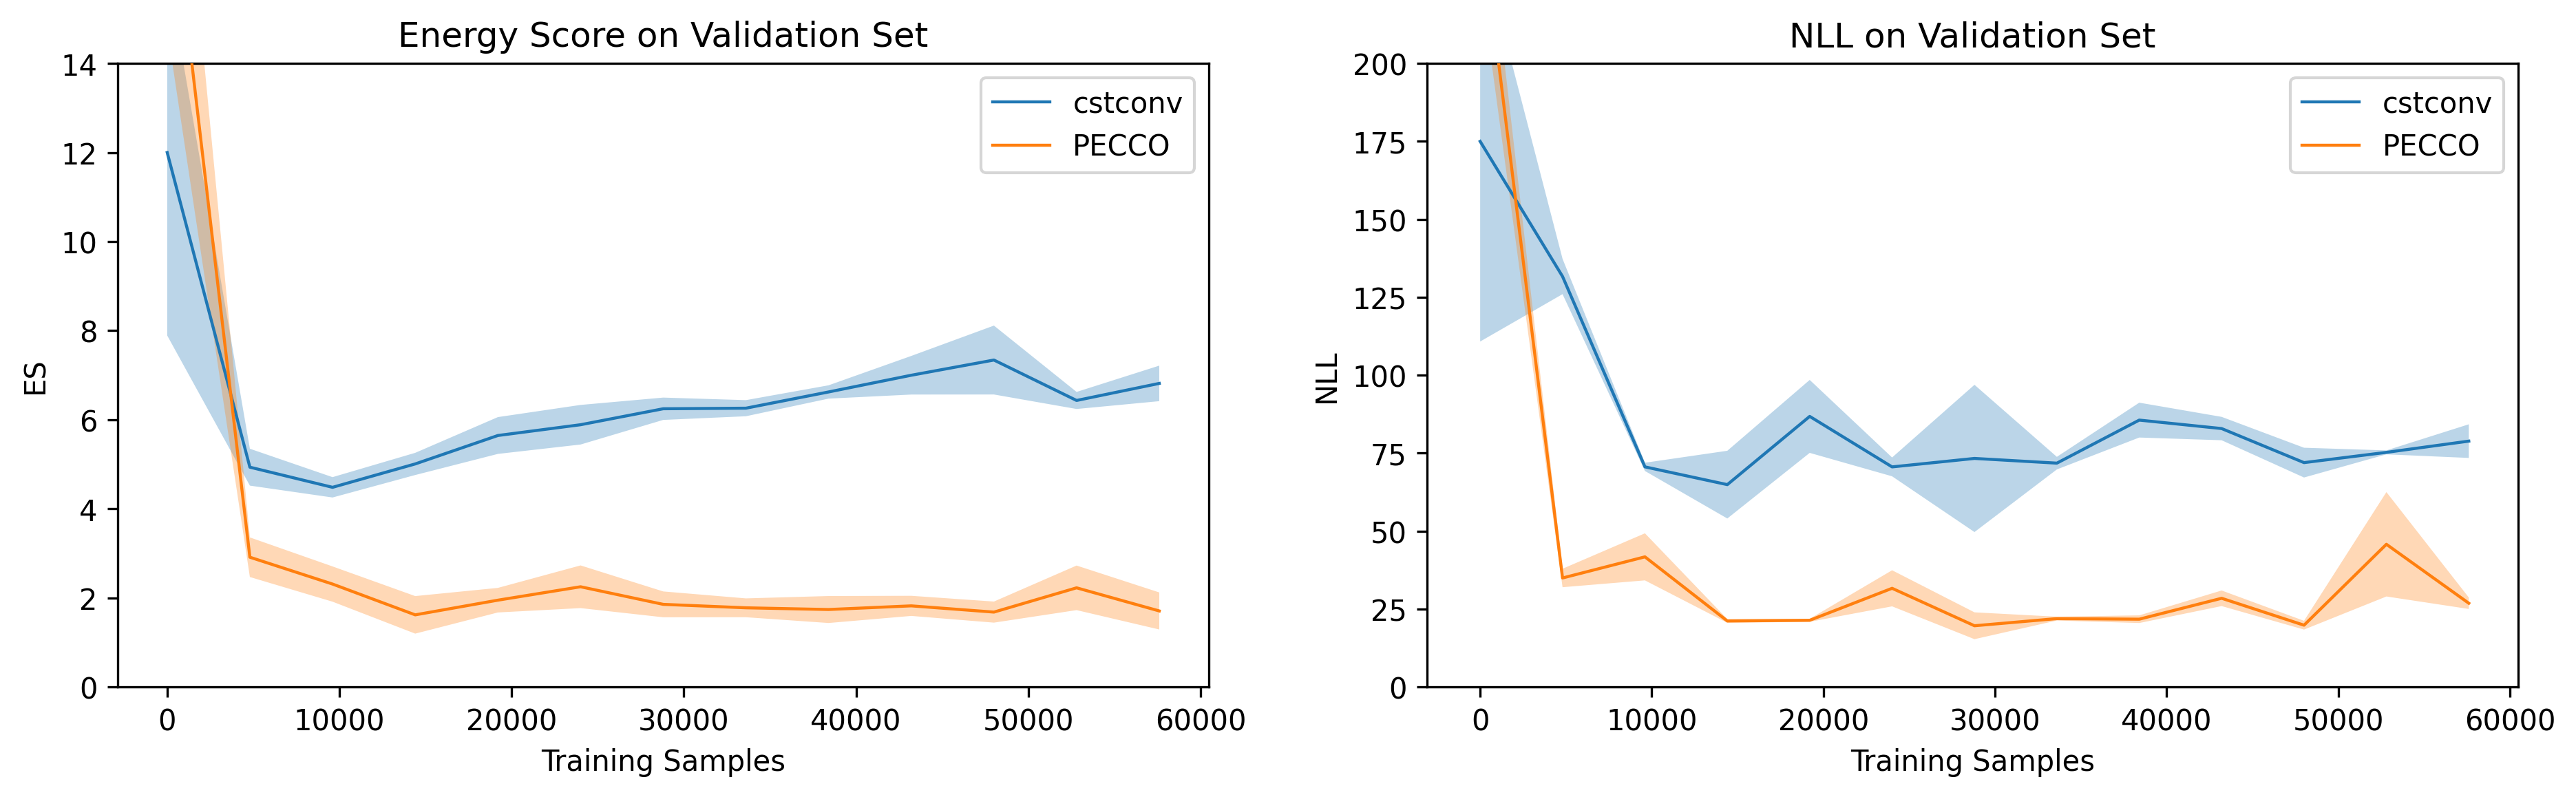
\includegraphics[width=.9\textwidth]{equivariance/figs/dataeff.png}
    \caption{With equivariance, PECCO is able to achieve better energy score and NLL with fewer data samples, compared to its non-equivariant counterpart.}
    \label{fig:dataeff}
\end{figure}

\begin{table*}[h]
\centering\resizebox{\textwidth}{!}{
\begin{tabular}{ c|c c c| ccc } 
 \toprule
  \textbf{Model} & minADE${}_6 \downarrow$ & minFDE${}_6 \downarrow$ & MRS $\downarrow$ & Cov@1s(\%) & Cov@2s & Cov@3s\\ 
\midrule
Conformal LSTM & 2.45 \plusminus{0.09}  & 4.68 \plusminus{0.15} & 198.1 \plusminus{12.0} & 90.1 \plusminus{0.1} & 92.7 \plusminus{0.1} & 92.8 \plusminus{0.1}\\
Conformal ECCO & 1.96 \plusminus{0.06} & 4.32 \plusminus{0.10} & 220.9 \plusminus{8.1} & \textbf{90.0} \plusminus{0.1} & \textbf{90.1} \plusminus{0.1} & \textbf{90.0} \plusminus{0.1} \\
\midrule
PECCO   & \textbf{1.39} \plusminus{.02}  & \textbf{3.41} \plusminus{0.03} & \textbf{8.52} \plusminus{0.16} & 74.9 \plusminus{0.2} & 93.6 \plusminus{0.8} & 92.5 \plusminus{0.9}\\
\bottomrule
\end{tabular}}
\caption{Comparison with conformal prediction methods on Argoverse dataset. PECCO produces a parametric distribution with a tighter confidence region (small MRS), whereby achieving better regression accuracy while maintaining competitive coverage.}
\label{tab:conformal}
\end{table*}


\subsection{Model Analysis}
%
\paragraph{Comparison with data augmentation and cannonicalization.}
Data augmentation and cannonicalization are popular methods to implicitly exploit symmetry in trajectory data. In Table 4 we compare PECCO to its nonequivariant counterparts with the addition of data augmentation and cannonicalization. Equivariance dramatically improves prediction performance in all aspects, especially calibration.

\begin{table}
\centering 
\begin{tabular}{ c | c c c c } 
 \toprule
  & minA/FDE$_6$ & NLL & Cov(\%) \\ 
 \midrule
  CtsConv & 1.74 / 4.43  & 29.13 & 2.2 \\
+cannon & 1.66 / 4.28 & 17.46  &  4.5  \\
+aug & 1.67 / 4.23  & 11.81  &  17.1 \\
equivariant & \textbf{1.39} / \textbf{3.41} & \textbf{4.26}  & \textbf{87.5} \\
\bottomrule
 \end{tabular}
\caption{Data Augmentation Comparison on the Argoverse Dataset.}
\label{tab:aug-ablation}
\end{table}

\paragraph{Dynamics Integration Ablation.}
Dynamic integration (dyna) introduced in Section \ref{sec:dyn_inte} enforces the uncertainty to grow monotonically over time. As an ablative study, Table 5 show that PECCO with  dynamic integration has much better calibration compared to if without; for the Argoverse dataset, the improved calibration also informs better performance on minADE/FDE.

\begin{table}
\centering 
\begin{tabular}{ c|c c c  } 
\toprule
\textbf{Argoverse} & minA/FDE$_6$ & NLL & Cov(\%) \\ 
\midrule
no-dyna & 1.52 / 3.76 & 9.72  & 38.6 \\
dyna & \textbf{1.39} / \textbf{3.41} & \textbf{4.26}  &  \textbf{87.5} \\
\toprule
\textbf{Pedestrian} & minA/FDE$_6$ & NLL & Cov(\%) \\ 
\midrule
no-dyna & \textbf{0.72} / 2.12 & 4.71 & 39.6  \\
dyna & 0.73 / \textbf{1.98} & \textbf{2.37}  & \textbf{83.7} \\
\bottomrule
\end{tabular}
\caption{Dynamics Integration (dyna) Ablation: using dyna encourages the uncertainty to grow over time and improves coverage.}
\label{tab:dynamics-ablation}
\end{table}


\paragraph{Comparison with Conformal Prediction.}
%Conformal prediction is a uncertainty quantification method with theoretical guarantees on coverage without imposing any assumptions about the underlying distribution.
We compare to two conformal prediction baselines \cite{2021conformal} (Appendix \ref{app:conformal} for details) in Table 3. Conformal methods achieve guaranteed $\geq 90\%$ coverage, but suffer in prediction accuracy due to having to split training data for calibration. Since conformal prediction does not output a distribution, we use another proper scoring rule Mean Regional Score (2d extension of mean interval score in \cite{properscoring}, see Appendix B) as metric. The conformal regions are much larger (higher MRS), which is less desirable for downstream decision making tasks.
%see appendix \ref{app:conformal} for details and qualitative visualization.